\section{Subspaces of \texorpdfstring{$\R^n$}{Rn}}
\label{sec:subspaces-rn}

\begin{outcome}
  \begin{enumerate}
  \item Determine whether a subset of $\R^n$ is a subspace.
  \item Recognize that spans are subspaces of $\R^n$.
  \item Recognize that solution sets of homogeneous systems of
    equations are subspaces of $\R^n$.
  \end{enumerate}
\end{outcome}

As we saw earlier, the span of 0 vectors in $\R^n$ is a point, namely
the set $\set{\vect{0}}$. The span of one non-zero vector is a line
through the origin, and the span of two linearly independent vectors
is a plane through the origin.
\begin{center}
  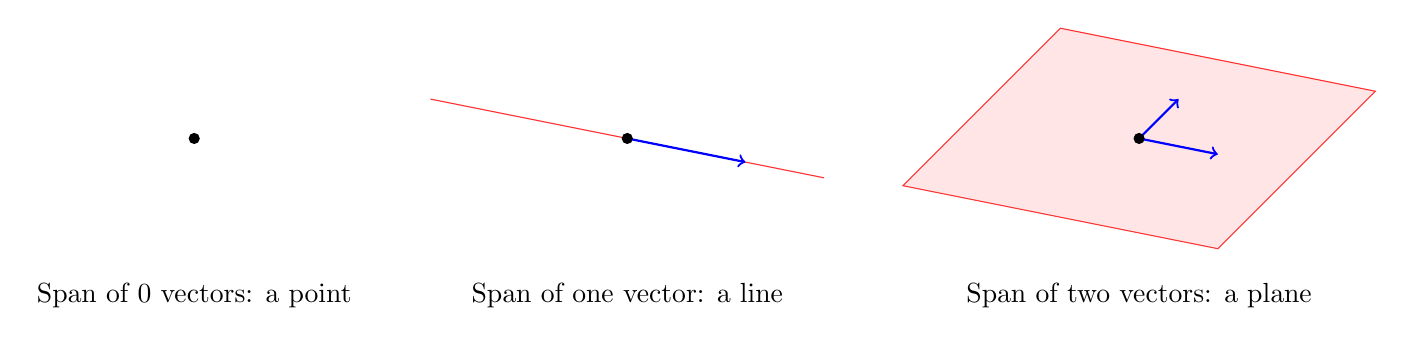
\begin{tikzpicture}
    \begin{scope}[xshift=-6cm]
      \draw[fill](0,0) circle [radius=1.8pt];
      \path(0,-2) node {Span of 0 vectors: a point};
    \end{scope}
    \begin{scope}[xshift=-0.5cm]
      \begin{scope}[x={(1cm,-0.2cm)},y={(0.5cm,0.5cm)}]
        \draw[red!80](-2.5,0) -- (2.5,0);
        \draw[->, thick, blue](0,0) -- +(1.5,0);
        \draw[fill](0,0) circle [radius=1.8pt];
      \end{scope}
      \path(0,-2) node {Span of one vector: a line};
    \end{scope}
    \begin{scope}[xshift=6cm]
      \begin{scope}[x={(1cm,-0.2cm)},y={(0.5cm,0.5cm)},z={(0cm,1cm)}]
        \filldraw[draw=red!80,fill=red!10](-2,-2,0) -- (2,-2,0) -- (2,2,0) -- (-2,2,0) -- cycle;
        \draw[->, thick, blue](0,0) -- +(0,1,0);
        \draw[->, thick, blue](0,0,0) -- +(1,0,0);
        \draw[fill](0,0) circle [radius=1.8pt];
      \end{scope}
      \path(0,-2) node {Span of two vectors: a plane};
    \end{scope}
  \end{tikzpicture}
\end{center}
We also call these sets, respectively, a {\em $0$-dimensional
  subspace}, a {\em $1$-dimensional subspace}, and a {\em
  $2$-dimensional subspace} of\/ $\R^n$. The purpose of this section is
to generalize this concept of subspace to arbitrary dimensions.

\begin{definition}{Subspace}{subspace}
  A subset $V$ of\/ $\R^n$ is called a \textbf{subspace}%
  \index{subspace!of Rn@of\/ $\R^n$} of\/ $\R^n$ if
  \begin{enumerate}
  \item $V$ contains the zero vector of\/ $\R^n$, i.e., $\vect{0}\in V$;
  \item $V$ is closed under addition, i.e., for all\/
    $\vect{u},\vect{w}\in V$, we have $\vect{u}+\vect{w}\in V$;
  \item $V$ is closed under scalar multiplication, i.e., for all\/
    $\vect{u}\in V$ and scalars $k$, we have\/ $k\,\vect{u}\in V$.
  \end{enumerate}
\end{definition}

Notice that the subset $V = \set{\vect{0}}$ is a subspace of\/ $\R^n$
(called the \textbf{zero subspace}%
\index{zero subspace}%
\index{subspace!zero subspace}). Every line or plane through the
origin is a subspace. Moreover, the entire space $\R^n$ is a subspace
of itself. A subspace that is not the zero subspace or the entire
space $\R^n$ is referred to as a \textbf{proper subspace}%
\index{proper subspace}%
\index{subspace!proper} of\/ $\R^n$.

\begin{proposition}{Spans are subspaces}{span-subspace}
  Let $\vect{u}_1,\ldots,\vect{u}_k$ be vectors in $\R^n$. Then
  $\sspan\set{\vect{u}_1,\ldots,\vect{u}_k}$ is a subspace of
  $\R^n$.%
  \index{subspace!span is a subspace}%
  \index{span!as a subspace}%
  \index{vector!span!as a subspace}%
\end{proposition}

\begin{proof}
  Let $S=\sspan\set{\vect{u}_1,\ldots,\vect{u}_k}$. To verify that $S$
  is a subspace of\/ $\R^n$, we must check that the three conditions
  of Definition~\ref{def:subspace} hold.
  \begin{itemize}
  \item We have $\vect{0}\in S$ because
    $\vect{0}=0\vect{u}_1+\ldots+0\vect{u}_k$.
  \item Suppose $\vect{u},\vect{w}\in S$.
    By definition of span, there exist scalars $a_1,\ldots,a_k$ and
    $b_1,\ldots,b_k$ such that
    $\vect{u}=a_1\,\vect{u}_1+\ldots+a_k\,\vect{u}_k$ and
    $\vect{w}=b_1\,\vect{u}_1+\ldots+b_k\,\vect{u}_k$.
    Therefore,
    \begin{equation*}
      \vect{u}+\vect{w} = \vect{u}=(a_1+b_1)\vect{u}_1+\ldots+(a_k+b_k)\vect{u}_k.
    \end{equation*}
    It follows that
    $\vect{u}+\vect{w}\in S=\sspan\set{\vect{u}_1,\ldots,\vect{u}_k}$,
    so that $S$ is closed under addition.
  \item Suppose $\vect{u}\in S$ and $t$ is a scalar. Then by
    definition of span, there exists scalars $a_1,\ldots,a_k$ such
    that $\vect{u}=a_1\,\vect{u}_1+\ldots+a_k\,\vect{u}_k$. Then
    \begin{equation*}
      t\,\vect{u}=(ta_1)\vect{u}_1+\ldots+(ta_k)\vect{u}_k,
    \end{equation*}
    and thus $t\,\vect{u}\in S$. It follows that $S$ is closed under
    scalar multiplication.
  \end{itemize}
  Since $S=\sspan\set{\vect{u}_1,\ldots,\vect{u}_k}$ satisfies all
  three conditions, it follows that it is a subspace of\/ $\R^n$.
\end{proof}

\begin{example}{A line in $\R^3$}{line-subspace}
  In $\R^3$, let $L$ be the line through the origin that is
  parallel to the vector
  \begin{equation*}
    {\vect{d}}= \begin{mymatrix}{r} -5 \\ 1 \\ -4 \end{mymatrix}.
  \end{equation*}
  Show that $L$ is a subspace of\/ $\R^3$.
\end{example}

\begin{solution}
  The line $L$ is simply the span of the vector $\vect{d}$, i.e.,
  $L=\sspan\set{\vect{d}}$. Therefore, it is a subspace by
  Proposition~\ref{prop:span-subspace}.
\end{solution}

\begin{proposition}{Solution space of a homogeneous system of equations}{solution-space}
  Consider a homogeneous system of equations $A\vect{x} = \vect{0}$,
  where $A$ is an $m\times n$-matrix. Then the set of solutions,
  \begin{equation*}
    V=\set{\vect{x}\in\R^n \mid A\vect{x} = \vect{0}},
  \end{equation*}
  is a subspace of\/ $\R^n$. It is called the \textbf{solution space} of
  the system.%
  \index{subspace!solution space of a homogeneous system}%
  \index{homogeneous system!solution space}%
  \index{solution space}%
  \index{system of linear equations!homogeneous!solution space}%
\end{proposition}

\begin{proof}
  To show that $V$ is a subspace of\/ $\R^n$, we check the three
  conditions of Definition~\ref{def:subspace}.
  \begin{itemize}
  \item We have $\vect{0}\in V$ because $A\vect{0}=\vect{0}$.
  \item To show that $V$ is closed under addition, suppose
    $\vect{u},\vect{w}\in V$.  Then by definition of $V$,
    $A\vect{u}=\vect{0}$ and $A\vect{w}=\vect{0}$.  Therefore,
    \begin{equation*}
      A(\vect{u}+\vect{w}) = A\vect{u} + A\vect{w} = \vect{0}+\vect{0}
      = \vect{0}.
    \end{equation*}
    It follows that $\vect{u}+\vect{w}\in V$.
  \item To show that $V$ is closed under scalar multiplication,
    suppose $\vect{u}\in V$ and $t$ is a scalar. Then by definition of
    $V$, we have $A\vect{u}=\vect{0}$. It follows that
    \begin{equation*}
      A(t\,\vect{u}) = t(A\vect{u}) = t\,\vect{0} = \vect{0}.
    \end{equation*}
    Therefore, $t\,\vect{u}\in V$.
  \end{itemize}
  Since the solution space
  $V=\set{\vect{x}\in\R^n \mid A\vect{x} = \vect{0}}$ satisfies all
  three conditions, it is a subspace of\/ $\R^n$.
\end{proof}

\begin{example}{A plane in $\R^3$}{plane-subspace}
  Show that the plane $2x+3y-z=0$ is a subspace of\/ $\R^3$.
\end{example}

\begin{solution}
  Since $2x+3y-z=0$ is a homogeneous equation, its solution space
  \begin{equation*}
    \set{\left.\begin{mymatrix}{c}x\\y\\z\end{mymatrix}~\right\vert~ 2x+3y-z=0}
  \end{equation*}
  is a subspace of\/ $\R^3$ by Proposition~\ref{prop:solution-space}.
\end{solution}

\begin{example}{Non-examples}{subspace-non-examples}
  Which of the following are subspaces of\/ $\R^3$?
  \begin{enumialphparenastyle}
    \begin{enumerate}
    \item The line
      \begin{equation*}
        \begin{mymatrix}{c} x \\ y \\ z \end{mymatrix}
        = \begin{mymatrix}{c} 1 \\ 2 \\ 3 \end{mymatrix}
        + t\begin{mymatrix}{c} 1 \\ 0 \\ 1 \end{mymatrix}.
      \end{equation*}
    \item The plane $2x+3y-z=5$.
    \item The set of vectors
      \begin{equation*}
        W=\set{\left.\begin{mymatrix}{c}x\\y\\z\end{mymatrix}
            ~\right\vert~ x,y,z\geq 0}.
      \end{equation*}
      ~
    \end{enumerate}
  \end{enumialphparenastyle}
\end{example}

\begin{solution}
  None of them are subspaces. Neither the line (a) nor the plane (b)
  contains the origin $\vect{0}$, so they fail to satisfy the first
  condition of subspaces. The set of vectors in (c) contains
  $\vect{0}$. It is also closed under addition. However, it fails to
  be closed under scalar multiplication. For example, let
  $\vect{u}=\mat{1,1,1}^T$. Then $\vect{u}\in W$, but
  $(-1)\vect{u}\not\in W$.
\end{solution}

